\documentclass[11pt]{article}

\usepackage[margin=1in]{geometry}
\usepackage{amsmath, amssymb, amsthm}
\usepackage{booktabs}
\usepackage{tikz}
\usepackage{caption}
\usepackage{subcaption}
\usepackage{hyperref}
\usetikzlibrary{positioning, arrows.meta, automata, backgrounds, fit, calc, plotmarks}

\theoremstyle{definition}
\newtheorem{definition}{Definition}[section]
\newtheorem{example}{Example}[section]
\theoremstyle{plain}
\newtheorem{proposition}[definition]{Proposition}
\newtheorem{lemma}[definition]{Lemma}
\theoremstyle{remark}
\newtheorem{remark}[definition]{Remark}

% numbers generated by compute-example.R
\newcommand{\dataN}{10}
\newcommand{\dataLambda}{4.605}
\newcommand{\dataX}{0.2,\ -0.1,\ 0.1,\ 0.0,\ 5.1,\ 4.9,\ 5.0,\ 5.2,\ 4.8,\ 5.0}
\newcommand{\dataSigma}{1,\ 1,\ 2,\ 2,\ 2,\ 3,\ 1,\ 4,\ 4,\ 4}
\newcommand{\sse}{0.150}
\newcommand{\penObj}{4.755}
\newcommand{\lopartLoss}{-150.010}
\newcommand{\lopartLossAbs}{150.010}
\newcommand{\sumsq}{150.160}
\newcommand{\numChanges}{1}
\newcommand{\pathStates}{normal,normal,normal,normal,noChange,normal,normal,normal,normal,normal}

\newcommand{\pointsCoords}{(1,0.200)(2,-0.100)(3,0.100)(4,0.000)(5,5.100)(6,4.900)(7,5.000)(8,5.200)(9,4.800)(10,5.000)}

\newcommand{\fitCoords}{(0.50,0.050)(4.50,0.050)(4.50,5.000)(10.50,5.000)}

\newcommand{\sigmaRows}{
1 & 0.2 & unlabeled & 1 & $n\!\to\!n$ null,\ $n\!\to\!n$ std \\
2 & -0.1 & unlabeled & 1 & $n\!\to\!n$ null,\ $n\!\to\!n$ std \\
3 & 0.1 & in pos. & 2 & $n\!\to\!n$ null,\ $c\!\to\!c$ null,\ $n\!\to\!c$ std \\
4 & 0.0 & in pos. & 2 & $n\!\to\!n$ null,\ $c\!\to\!c$ null,\ $n\!\to\!c$ std \\
5 & 5.1 & in pos. & 2 & $n\!\to\!n$ null,\ $c\!\to\!c$ null,\ $n\!\to\!c$ std \\
6 & 4.9 & end pos. & 3 & $n\!\to\!n$ std,\ $c\!\to\!n$ null \\
7 & 5.0 & unlabeled & 1 & $n\!\to\!n$ null,\ $n\!\to\!n$ std \\
8 & 5.2 & in neg. & 4 & $n\!\to\!n$ null \\
9 & 4.8 & in neg. & 4 & $n\!\to\!n$ null \\
10 & 5.0 & in neg. & 4 & $n\!\to\!n$ null \\
}

\newcommand{\qRows}{
1 & 0.2 & 0.00 & $+\infty$ \\
2 & -0.1 & 0.05 & $+\infty$ \\
3 & 0.1 & 0.05 & 4.65 \\
4 & 0.0 & 0.05 & 4.65 \\
5 & 5.1 & 20.45 & 4.66 \\
6 & 4.9 & 4.68 & $+\infty$ \\
7 & 5.0 & 4.68 & $+\infty$ \\
8 & 5.2 & 4.71 & $+\infty$ \\
9 & 4.8 & 4.76 & $+\infty$ \\
10 & 5.0 & 4.76 & $+\infty$ \\
}

\newcommand{\segRows}{
1 & [1,4] & 0.050 \\
2 & [5,10] & 5.000 \\
}

\newcommand{\oracleRows}{
changepoints & $\{4,10\}$ & $\{4,10\}$ \\
segment means & $0.050,\,5.000$ & $0.050,\,5.000$ \\
residual SSE & $0.150$ & $150.160 - 150.010 = 0.150$ \\
}


\newcommand{\Rmap}{\sigma}
\newcommand{\Op}{\mathcal{O}}

\title{\textbf{Time-Dependent Constraints in \texttt{gfpop}}\\[2pt]
\large A mathematical description of the midterm deliverable}
\author{}
\date{}

\begin{document}
\maketitle
\vspace{-3em}

\begin{abstract}
\noindent \texttt{gfpop} solves penalized change-point problems under a
user-specified constraint graph, but the \emph{same} graph is imposed at every
time step. This note develops the mathematics of an extension in which the
active constraints may depend on the time index through a \emph{rule map}. We
formalise the recursion, prove that the extension is a strict generalisation
(it reduces to ordinary \texttt{gfpop} when the rule is constant) and that
unreachable states are handled automatically by the existing infinity
arithmetic. We then encode two labelled change-point models as time-dependent
graphs --- the Gaussian LOPART model and an up-down peak model that no current
R package expresses --- and trace the full dynamic program on a ten-point
dataset, cross-checked exactly against \texttt{LOPART::LOPART()}. Every number
in Section~\ref{sec:run} is produced by an accompanying R script.
\end{abstract}

%======================================================================
\section{Motivation}\label{sec:motivation}

Consider the following $n=\dataN$ observations (our running example throughout):
\[
  x = (\dataX).
\]
An analyst has annotated two regions: a \emph{positive} label on $[3,6]$
asserting that \emph{exactly one} change occurs there, and a \emph{negative}
label on $[8,10]$ asserting that \emph{no} change occurs there (Figure~\ref{fig:data}).

\begin{figure}[h]
\centering
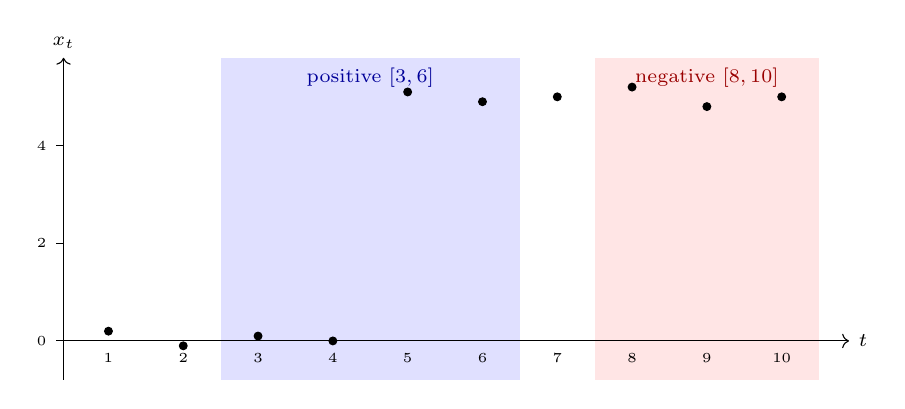
\begin{tikzpicture}[x=0.95cm, y=0.62cm]
  \fill[blue!12] (2.5,-0.8) rectangle (6.5,5.8);
  \fill[red!10]  (7.5,-0.8) rectangle (10.5,5.8);
  \node[blue!60!black, font=\scriptsize] at (4.5,5.4) {positive $[3,6]$};
  \node[red!60!black, font=\scriptsize] at (9,5.4) {negative $[8,10]$};
  \draw[->] (0.4,0) -- (10.9,0) node[right, font=\scriptsize] {$t$};
  \draw[->] (0.4,-0.8) -- (0.4,5.8) node[above, font=\scriptsize] {$x_t$};
  \foreach \y in {0,2,4} { \draw (0.3,\y)--(0.4,\y); \node[left, font=\tiny] at (0.3,\y) {\y}; }
  \foreach \t in {1,...,10} { \node[below, font=\tiny] at (\t,-0.05) {\t}; }
  \draw plot[only marks, mark=*, mark size=1.4pt] coordinates {\pointsCoords};
\end{tikzpicture}
\caption{The running dataset. Shaded: the positive label (blue, one change
expected) and the negative label (red, no change expected).}
\label{fig:data}
\end{figure}

The data clearly step up once, near $t=4$--$5$. Standard penalized
segmentation would find this change from the data alone; but it has no way to
\emph{use} the analyst's labels, which encode where changes are or are not
permitted. \texttt{gfpop} can encode rich structural constraints through a
graph, yet that graph is fixed across time, whereas a label is intrinsically
\emph{positional}: it constrains some indices and not others. Bridging that gap
is the subject of this note. The motivating application is genomic peak
detection, where experts label regions of a coverage profile as containing a
peak or not, and one wants a segmentation consistent with those labels.

%======================================================================
\section{Background: penalized change-point detection}\label{sec:back-fpop}

Write a segmentation of $x_{1:n}$ through its vector of segment means
$\mu_{1:n}$, constant on each segment, with a change at $t$ whenever
$\mu_t \neq \mu_{t+1}$. For Gaussian (least-squares) loss the penalized
objective is
\begin{equation}\label{eq:objective}
  \min_{\mu_{1:n}} \ \sum_{t=1}^n (x_t-\mu_t)^2
    \ +\ \lambda \, \bigl|\{\, t< n : \mu_t \neq \mu_{t+1}\,\}\bigr|,
\end{equation}
with penalty $\lambda>0$ discouraging spurious changes. Optimal partitioning
solves \eqref{eq:objective} by the dynamic program that tracks, as a function
of the last segment's mean, the best cost of a prefix. \texttt{gfpop} keeps the
exact \emph{cost function}
\[
  Q_t(\mu) \;=\; \min\bigl\{\, \text{penalized cost of } x_{1:t}
      \ \text{with last mean } \mu \,\bigr\},
\]
a piecewise quadratic in $\mu$. Two operations recur: adding a data point,
$Q(\mu)\mapsto Q(\mu)+(x_t-\mu)^2$ (a quadratic shift), and committing a change,
$Q \mapsto \min_\nu Q(\nu) + \lambda$ (a constant). Functional pruning keeps only
the lower envelope of the candidate quadratics; the minimum over $\mu$ is read
from that envelope (Figure~\ref{fig:envelope}).

\begin{figure}[h]
\centering
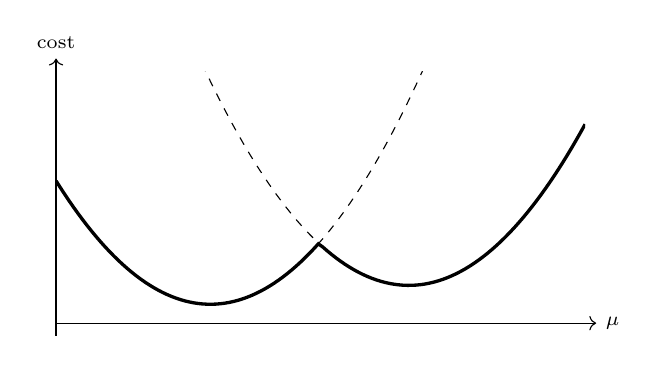
\begin{tikzpicture}[x=1.4cm, y=0.8cm]
  \draw[->] (-2.4,0) -- (2.5,0) node[right, font=\scriptsize] {$\mu$};
  \draw[->] (-2.4,-0.2) -- (-2.4,4.2) node[above, font=\scriptsize] {cost};
  \begin{scope}
    \clip (-2.4,-0.2) rectangle (2.4,4);
    \draw[dashed] plot[domain=-2.4:2.4, samples=80] (\x,{(\x+1)^2+0.3});
    \draw[dashed] plot[domain=-2.4:2.4, samples=80] (\x,{(\x-0.8)^2+0.6});
    \draw[very thick] plot[domain=-2.4:2.4, samples=120]
      (\x,{min((\x+1)^2+0.3,(\x-0.8)^2+0.6)});
  \end{scope}
\end{tikzpicture}
\caption{Two candidate quadratics (dashed) and their lower envelope (solid).
$Q_t(\mu)$ is such an envelope; $\min_\mu Q_t(\mu)$ is its lowest point.}
\label{fig:envelope}
\end{figure}

\begin{example}\label{ex:micro}
On the first three points $x_1,x_2,x_3 = 0.2,-0.1,0.1$, if no change is taken,
$Q_3(\mu)=(0.2-\mu)^2+(-0.1-\mu)^2+(0.1-\mu)^2 = 3\mu^2-0.4\mu+0.06$, minimised
at $\bar x=0.0\overline{6}$ with value $\approx 0.047$ (the $t=3$, ``normal''
entry of Table~\ref{tab:Q}).
\end{example}

%======================================================================
\section{Background: the \texttt{gfpop} graph formalism}\label{sec:back-graph}

\begin{definition}[Constraint graph]
A constraint graph is a directed multigraph $G=(S,E)$ on a finite set of states
$S$. Each edge $e=(s\to s')$ has a type in $\{\texttt{null},\texttt{std},
\texttt{up},\texttt{down}\}$ and a penalty $\beta_e\ge 0$. An edge acts on a cost
function by an operator $\Op_e$:
\[
  \Op_{\texttt{null}}(Q)=Q,\qquad
  \Op_{\texttt{std}}(Q)=\min_\nu Q(\nu)+\beta_e,
\]
while \texttt{up}/\texttt{down} additionally impose $\mu'\ge\nu$ / $\mu'\le\nu$
on the committed change.
\end{definition}

A state carries one cost function $Q_t^{s}$ per time. The recursion couples
states through the edges: for each destination $s'$,
\begin{equation}\label{eq:gfpop-rec}
  Q_{t}^{s'}(\mu) \;=\; \Bigl[\ \min_{e=(s\to s')\in E}\ \Op_e\bigl(Q_{t-1}^{s}\bigr)(\mu)\ \Bigr]
      \;+\; (x_{t}-\mu)^2 ,
\end{equation}
initialised at $t=1$ with $Q_1^{s}(\mu)=(x_1-\mu)^2$ for the start state and
$+\infty$ otherwise. Figure~\ref{fig:graphs} shows the two graphs we build on.

\begin{figure}[h]
\centering
\begin{subfigure}{0.35\textwidth}\centering
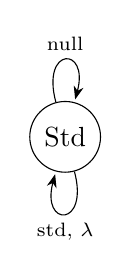
\begin{tikzpicture}[->,>=Stealth, node distance=2cm, on grid, auto]
  \node[state] (S) {Std};
  \path (S) edge[loop above] node[font=\scriptsize]{null} (S)
            edge[loop below] node[font=\scriptsize]{std, $\lambda$} (S);
\end{tikzpicture}
\caption{\texttt{std}: one state.}
\end{subfigure}\hspace{2em}
\begin{subfigure}{0.45\textwidth}\centering
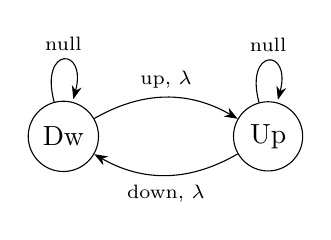
\begin{tikzpicture}[->,>=Stealth, node distance=2.6cm, on grid, auto]
  \node[state] (D) {Dw};
  \node[state] (U) [right=of D] {Up};
  \path (D) edge[loop above] node[font=\scriptsize]{null} (D)
        (U) edge[loop above] node[font=\scriptsize]{null} (U)
        (D) edge[bend left]  node[font=\scriptsize]{up, $\lambda$} (U)
        (U) edge[bend left]  node[font=\scriptsize]{down, $\lambda$} (D);
\end{tikzpicture}
\caption{\texttt{updown}: two states.}
\end{subfigure}
\caption{Standard \texttt{gfpop} graphs. Self-loops (\texttt{null}) continue a
segment; other edges (\texttt{std}/\texttt{up}/\texttt{down}) commit a change.}
\label{fig:graphs}
\end{figure}

%======================================================================
\section{The extension: time-dependent constraints}\label{sec:extension}

The single premise of \eqref{eq:gfpop-rec} we relax is that the minimisation
ranges over \emph{all} of $E$ at every step.

\begin{definition}[Rule map and active set]\label{def:rule}
Fix $R$ rules. A \emph{rule map} is a function $\Rmap:\{1,\dots,n\}\to\{1,\dots,R\}$.
Each edge $e$ carries a label $r(e)\in\{1,\dots,R\}\cup\{\textsc{na}\}$. The
\emph{active set} at time $t$ is
\[
  E_t \;=\; \{\, e\in E \ :\ r(e)=\textsc{na}\ \text{ or }\ r(e)=\Rmap(t)\,\}.
\]
Edges labelled \textsc{na} are always active; the others switch on only at the
steps their rule selects. The recursion is \eqref{eq:gfpop-rec} with $E$
replaced by $E_t$.
\end{definition}

Equivalently, one time-independent graph is \emph{sliced} per step: at time $t$
the solver sees the subgraph $(S,E_t)$. Figure~\ref{fig:timeexp} shows two
different slices of the same graph.

\begin{figure}[h]
\centering
\begin{subfigure}{0.46\textwidth}\centering
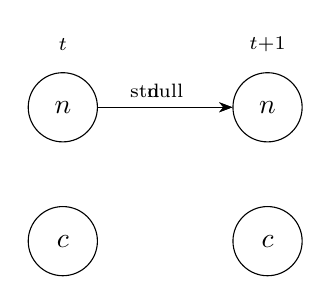
\begin{tikzpicture}[->,>=Stealth, node distance=1.7cm and 2.6cm, on grid, auto]
  \node[state] (n0) {$n$};
  \node[state] (c0) [below=of n0] {$c$};
  \node[state] (n1) [right=of n0] {$n$};
  \node[state] (c1) [below=of n1] {$c$};
  \node[font=\scriptsize] at ($(n0)+(0,0.8)$) {$t$};
  \node[font=\scriptsize] at ($(n1)+(0,0.8)$) {$t{+}1$};
  \path (n0) edge node[font=\scriptsize]{null} (n1)
        (n0) edge node[font=\scriptsize,pos=0.35]{std} (n1);
\end{tikzpicture}
\caption{$\Rmap(t{+}1)=1$ (unlabelled): only $n\to n$ edges.}
\end{subfigure}\hspace{1.5em}
\begin{subfigure}{0.46\textwidth}\centering
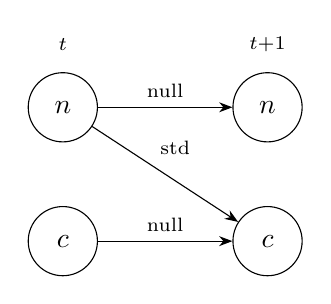
\begin{tikzpicture}[->,>=Stealth, node distance=1.7cm and 2.6cm, on grid, auto]
  \node[state] (n0) {$n$};
  \node[state] (c0) [below=of n0] {$c$};
  \node[state] (n1) [right=of n0] {$n$};
  \node[state] (c1) [below=of n1] {$c$};
  \node[font=\scriptsize] at ($(n0)+(0,0.8)$) {$t$};
  \node[font=\scriptsize] at ($(n1)+(0,0.8)$) {$t{+}1$};
  \path (n0) edge node[font=\scriptsize]{null} (n1)
        (n0) edge node[font=\scriptsize,pos=0.4]{std} (c1)
        (c0) edge node[font=\scriptsize]{null} (c1);
\end{tikzpicture}
\caption{$\Rmap(t{+}1)=2$ (in positive label): the $n\to c$ change turns on.}
\end{subfigure}
\caption{Two time slices of the LOPART graph ($n=$ normal, $c=$ noChange). The
active edge set changes with $\Rmap(t)$.}
\label{fig:timeexp}
\end{figure}

Two facts make this safe and cheap to add on top of the existing solver.

\begin{proposition}[Backward compatibility]\label{prop:bc}
If $\Rmap\equiv c$ is constant and every edge has $r(e)\in\{\textsc{na},c\}$,
then $E_t=E$ for all $t$ and the recursion coincides with ordinary
\texttt{gfpop}.
\end{proposition}
\begin{proof}
By Definition~\ref{def:rule}, $e\in E_t$ iff $r(e)=\textsc{na}$ or
$r(e)=\Rmap(t)=c$. Under the hypothesis every edge satisfies one of these, so
$E_t=E$ for every $t$, and \eqref{eq:gfpop-rec} is recovered verbatim. In
particular, supplying no rule (all edges \textsc{na}) leaves the output
unchanged.
\end{proof}

\begin{lemma}[Infinity semantics]\label{lem:inf}
Suppose no active edge enters state $s'$ at time $t$, i.e.\ $E_t$ contains no
edge $(\cdot\to s')$. Then $Q_t^{s'}\equiv+\infty$. Moreover both operators map
the constant $+\infty$ function to $+\infty$:
$\Op_{\texttt{null}}(+\infty)=+\infty$ and
$\Op_{\texttt{std}}(+\infty)=\min_\nu(+\infty)+\beta=+\infty$.
\end{lemma}
\begin{proof}
The bracketed minimum in \eqref{eq:gfpop-rec} is over the empty set, hence
$+\infty$; adding $(x_t-\mu)^2$ leaves $+\infty$. The operator identities are
immediate. Consequently an unreachable state contributes $+\infty$ to every
downstream minimisation and is silently ignored, with no case distinction.
\end{proof}

\begin{remark}
Lemma~\ref{lem:inf} is why the extension required \emph{no} change to
\texttt{gfpop}'s constraint operators (including the intricate
\texttt{up}/\texttt{down} code): skipping an inactive edge simply leaves its
destination at the $+\infty$ the solver already initialises, and the existing
arithmetic propagates it correctly.
\end{remark}

%======================================================================
\section{Model I: LOPART as a 4-rule, 2-state graph}\label{sec:lopart}

LOPART (Hocking \& Srivastava) performs Gaussian change-point detection subject
to labels: a positive region must contain exactly one change, a negative region
none. We reproduce it with states $S=\{\texttt{normal},\texttt{noChange}\}$ and
four rules, one per label context. The lock state \texttt{noChange} records that
the single change permitted in a positive region has been spent.

\begin{figure}[h]
\centering
\newcommand{\panel}[2]{%
\begin{tikzpicture}[->,>=Stealth, node distance=1.5cm, on grid, baseline]
  \node[state, minimum size=6mm, font=\scriptsize] (n) {$n$};
  \node[state, minimum size=6mm, font=\scriptsize] (c) [right=of n] {$c$};
  #2
\end{tikzpicture}}
\begin{subfigure}{0.24\textwidth}\centering
\panel{1}{\path (n) edge[loop above] node[font=\tiny]{null,std} (n);}
\caption{R1 unlabelled}
\end{subfigure}
\begin{subfigure}{0.24\textwidth}\centering
\panel{2}{\path (n) edge[loop above] node[font=\tiny]{null} (n)
                (c) edge[loop above] node[font=\tiny]{null} (c)
                (n) edge node[font=\tiny]{std} (c);}
\caption{R2 in positive}
\end{subfigure}
\begin{subfigure}{0.24\textwidth}\centering
\panel{3}{\path (n) edge[loop above] node[font=\tiny]{std} (n)
                (c) edge node[font=\tiny,above]{null} (n);}
\caption{R3 end positive}
\end{subfigure}
\begin{subfigure}{0.24\textwidth}\centering
\panel{4}{\path (n) edge[loop above] node[font=\tiny]{null} (n);}
\caption{R4 in negative}
\end{subfigure}
\caption{Rule filmstrip for LOPART: the active subgraph under each rule
($n=$ normal, $c=$ noChange).}
\label{fig:lopart-film}
\end{figure}

The label-to-rule map assigns each unlabelled index rule $1$; inside a positive
region, rule $2$, except its last index which gets rule $3$; inside a negative
region, rule $4$.

\begin{proposition}[Encoding correctness]\label{prop:lopart}
Under the filmstrip of Figure~\ref{fig:lopart-film}, the feasible state paths are
exactly the segmentations in which every positive region carries exactly one
change and every negative region none.
\end{proposition}
\begin{proof}[Proof sketch]
Enter a positive region in \texttt{normal}. Rule $2$ offers $n\to n$
(\texttt{null}, no change) or the single $n\to c$ (\texttt{std}, one change);
once in $c$ only $c\to c$ (\texttt{null}) is available, so at most one change
occurs. The region's last index uses rule $3$, whose only options are
$n\to n$ \texttt{std} (force the change if still in $n$) or $c\to n$
\texttt{null} (release if the change was already taken); there is no
$n\to n$ \texttt{null}, so the path cannot leave the region with zero changes.
Hence exactly one. A negative region (rule $4$) offers only $n\to n$
\texttt{null}: no change. Unlabelled steps (rule $1$) are the standard model.
Reading the construction backwards recovers a state path from any label-feasible
segmentation, giving the bijection.
\end{proof}

\begin{lemma}[Loss identity]\label{lem:loss}
Let $C_{\mathrm{gf}}=\sum_t (x_t-\hat\mu_t)^2$ be \texttt{gfpop}'s reported
residual cost and $L$ be \texttt{LOPART}'s reported \texttt{total\_loss} on the
same fit. Then $C_{\mathrm{gf}} = \sum_t x_t^2 + L$.
\end{lemma}
\begin{proof}
The two implementations minimise the same penalized objective and hence agree on
the optimal segmentation; they differ only in the additive constant reported as
``loss''. \texttt{LOPART} omits the data-only term $\sum_t x_t^2$ (independent of
$\mu$), so its loss equals $C_{\mathrm{gf}}-\sum_t x_t^2$. Rearranging gives the
identity, verified numerically in Table~\ref{tab:oracle}
($\sse = \sumsq - \lopartLossAbs$).
\end{proof}

%======================================================================
\section{Model II: up-down with labels (6 rules, 4 states)}\label{sec:updown}

The same mechanism expresses a model that, to our knowledge, no current R
package provides: labelled \emph{peak} detection under an up-down constraint.
Here a peak is a rise (\texttt{up}) followed later by a fall (\texttt{down}).
States are $\{\texttt{Dw},\texttt{Up},\texttt{noChangeUp},\texttt{noChangeDw}\}$,
the two lock states playing the role of \texttt{noChange} for each direction.

Peak-detection labels come in two positive flavours --- \texttt{peakStart}
(exactly one \texttt{up}) and \texttt{peakEnd} (exactly one \texttt{down}) ---
plus \texttt{noPeaks} (flat). Each is the LOPART \emph{(in, end)} pair applied to
one direction, giving $2+2$ positive rules plus unlabelled and \texttt{noPeaks}:
six in total. A single design point makes the end rules well-defined: the forced
change lands directly in the released state ($\texttt{Dw}\to\texttt{Up}$,
$\texttt{Up}\to\texttt{Dw}$) rather than in a lock, so one index performs one
action.

\begin{figure}[h]
\centering
\newcommand{\upanel}[1]{%
\begin{tikzpicture}[->,>=Stealth, node distance=1.15cm, on grid, baseline]
  \node[state, minimum size=5mm, inner sep=0, font=\tiny] (D) {Dw};
  \node[state, minimum size=5mm, inner sep=0, font=\tiny] (U) [right=1.6cm of D] {Up};
  \node[state, minimum size=5mm, inner sep=0, font=\tiny] (cu) [below=of D] {$c_u$};
  \node[state, minimum size=5mm, inner sep=0, font=\tiny] (cd) [below=of U] {$c_d$};
  #1
\end{tikzpicture}}
\begin{subfigure}{0.32\textwidth}\centering
\upanel{\path (D) edge[loop above] node[font=\tiny]{nl} (D)
              (U) edge[loop above] node[font=\tiny]{nl} (U)
              (D) edge[bend left] node[font=\tiny]{up} (U)
              (U) edge[bend left] node[font=\tiny]{dn} (D);}
\caption{R1 unlabelled}
\end{subfigure}
\begin{subfigure}{0.32\textwidth}\centering
\upanel{\path (D) edge[loop above] node[font=\tiny]{nl} (D)
              (D) edge node[font=\tiny]{up} (cu)
              (cu) edge[loop below] node[font=\tiny]{nl} (cu);}
\caption{R3 in peakStart}
\end{subfigure}
\begin{subfigure}{0.32\textwidth}\centering
\upanel{\path (D) edge node[font=\tiny]{up} (U)
              (cu) edge node[font=\tiny,pos=0.4]{nl} (U);}
\caption{R4 end peakStart}
\end{subfigure}
\caption{Three of the six up-down panels ($c_u=$ noChangeUp, $c_d=$ noChangeDw;
nl $=$ null). Rules 5--6 mirror 3--4 with \texttt{Up}$\to$\texttt{Dw} via
\texttt{down} and $c_d$; rule~2 (\texttt{noPeaks}) keeps only the two
\texttt{null} self-loops.}
\label{fig:updown-film}
\end{figure}

Lacking an oracle, this model is validated \emph{structurally}: on synthetic
labelled peaks it must place exactly one change in each \texttt{peakStart},
exactly one in each \texttt{peakEnd}, and none in any \texttt{noPeaks}; and with
every index unlabelled it must reproduce \texttt{graph(type="updown")} exactly.
Both hold in the test suite.

%======================================================================
\section{The full ten-step run}\label{sec:run}

We now trace Model~I on the dataset of Section~\ref{sec:motivation} with penalty
$\lambda = 2\log \dataN = \dataLambda$. The rule map is $\Rmap = (\dataSigma)$;
Table~\ref{tab:sigma} shows how each index's label context selects its active
edges.

\begin{table}[h]\centering\small
\begin{tabular}{ccccl}
\toprule
$t$ & $x_t$ & context & $\Rmap(t)$ & active edges ($n=$ normal, $c=$ noChange)\\
\midrule
\sigmaRows
\bottomrule
\end{tabular}
\caption{The rule map and the active edge set at each step.}
\label{tab:sigma}
\end{table}

\paragraph{The dynamic program.}
Table~\ref{tab:Q} lists the per-state minima $m_t^{s}=\min_\mu Q_t^{s}(\mu)$
(the penalized cost of the best prefix ending in state $s$ at time $t$),
computed by the functional recursion \eqref{eq:gfpop-rec}. The infinity pattern
of Lemma~\ref{lem:inf} is visible directly: \texttt{noChange} is $+\infty$
before the positive label (nothing enters it), becomes finite only for
$t\in\{3,4,5\}$, and returns to $+\infty$ once rule~3 releases the lock. At
$t=5$, staying in \texttt{normal} costs $20.45$ (the high point $x_5=5.1$ forced
into the low segment) whereas \texttt{noChange} costs only $4.66$ --- this is
exactly why the optimal path commits the change here.

\begin{table}[h]\centering\small
\begin{tabular}{cccc}
\toprule
$t$ & $x_t$ & $m_t^{\texttt{normal}}$ & $m_t^{\texttt{noChange}}$\\
\midrule
\qRows
\bottomrule
\end{tabular}
\caption{Functional minima per state. Penalized costs (a committed change adds
$\lambda$); $+\infty$ marks an unreachable state.}
\label{tab:Q}
\end{table}

\paragraph{The optimal path.}
Backtracking the recursion gives the state trellis of
Figure~\ref{fig:trellis}: the path stays in \texttt{normal}, dips into
\texttt{noChange} at $t=5$ to absorb the single permitted change, and is
released back to \texttt{normal} at $t=6$.

\begin{figure}[h]
\centering
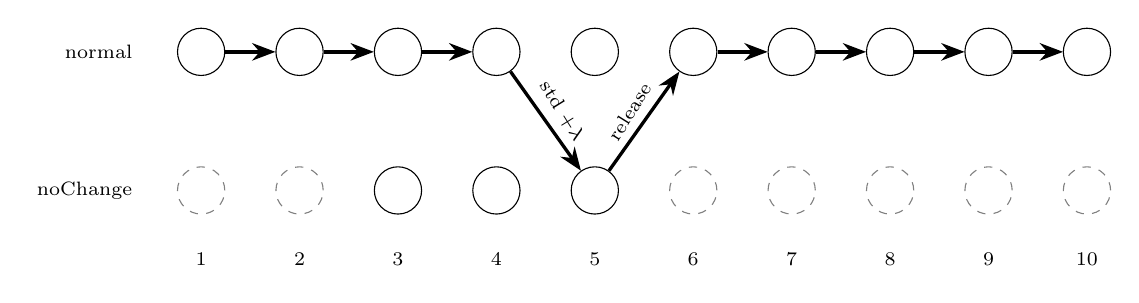
\begin{tikzpicture}[>=Stealth, xscale=1.25, yscale=1.1]
  % nodes
  \foreach \t in {1,...,10}{
    \node[draw, circle, minimum size=6mm, inner sep=0] (N\t) at (\t,0) {};
    \node[font=\scriptsize] at (\t,-2.4) {\t};
  }
  \foreach \t in {1,2,6,7,8,9,10}{
    \node[draw, circle, dashed, gray, minimum size=6mm, inner sep=0] (C\t) at (\t,-1.6) {};
  }
  \foreach \t in {3,4,5}{
    \node[draw, circle, minimum size=6mm, inner sep=0] (C\t) at (\t,-1.6) {};
  }
  \node[font=\scriptsize, left] at (0.4,0) {normal};
  \node[font=\scriptsize, left] at (0.4,-1.6) {noChange};
  % optimal path (thick)
  \foreach \a/\b in {1/2,2/3,3/4}{ \draw[very thick,->] (N\a)--(N\b); }
  \draw[very thick,->] (N4)--(C5) node[midway, sloped, font=\scriptsize, above] {std $+\lambda$};
  \draw[very thick,->] (C5)--(N6) node[midway, sloped, font=\scriptsize, above] {release};
  \foreach \a/\b in {6/7,7/8,8/9,9/10}{ \draw[very thick,->] (N\a)--(N\b); }
\end{tikzpicture}
\caption{Optimal state path. Solid \texttt{noChange} nodes ($t=3,4,5$) are
reachable; dashed ones are $+\infty$. The change at $t=4$ is the
$\texttt{normal}\to\texttt{noChange}$ \texttt{std} edge.}
\label{fig:trellis}
\end{figure}

\paragraph{The segmentation.}
The result is $\numChanges$ change, splitting the data into the segments of
Table~\ref{tab:seg}, drawn over the data in Figure~\ref{fig:fit}.

\begin{minipage}{0.42\textwidth}\centering
\small
\begin{tabular}{ccc}
\toprule
segment & range & mean\\
\midrule
\segRows
\bottomrule
\end{tabular}
\captionof{table}{Fitted segments.}
\label{tab:seg}
\end{minipage}\hfill
\begin{minipage}{0.55\textwidth}\centering
\begin{tikzpicture}[x=0.5cm, y=0.62cm]
  \draw[->] (0.4,0) -- (10.9,0) node[right, font=\scriptsize] {$t$};
  \draw[->] (0.4,-0.8) -- (0.4,5.8) node[above, font=\scriptsize] {$x_t$};
  \foreach \y in {0,2,4} { \draw (0.3,\y)--(0.4,\y); \node[left, font=\tiny] at (0.3,\y) {\y}; }
  \draw[very thick, gray] plot coordinates {\fitCoords};
  \draw plot[only marks, mark=*, mark size=1.2pt] coordinates {\pointsCoords};
\end{tikzpicture}
\captionof{figure}{Data and fitted piecewise-constant mean.}
\label{fig:fit}
\end{minipage}

\paragraph{Oracle cross-check.}
Running \texttt{LOPART::LOPART()} on the same data, labels and penalty gives an
identical fit (Table~\ref{tab:oracle}): same changepoints, same means, and the
residual cost matching through the constant of Lemma~\ref{lem:loss}.

\begin{table}[h]\centering\small
\begin{tabular}{lcc}
\toprule
 & \texttt{gfpop}$(\text{rule}=\Rmap)$ & \texttt{LOPART::LOPART()}\\
\midrule
\oracleRows
\bottomrule
\end{tabular}
\caption{Exact agreement with the oracle on the running example.}
\label{tab:oracle}
\end{table}

%======================================================================
\section{Validation summary and outlook}\label{sec:summary}

Three kinds of guarantee support the deliverable. \emph{Backward compatibility}
(Proposition~\ref{prop:bc}) is tested by running each labelled graph with an
all-unlabelled rule and checking it equals the corresponding standard graph
exactly. \emph{Oracle exactness} (Model~I) is tested against
\texttt{LOPART::LOPART()}: identical changepoints, means and cost up to the
constant of Lemma~\ref{lem:loss}. \emph{Structural invariants} (Model~II, which
has no oracle) check that each label region receives the mandated number of
changes. All three pass in continuous integration across Linux, macOS and
Windows.

The remaining work builds on this core: a user-facing vignette with a filmstrip
visualisation of the rule-sliced graph, performance benchmarks, and an extension
of the labelled models to Poisson loss. The mathematics above --- a rule map
selecting an active subgraph per step, with unreachable states absorbed by the
existing infinity arithmetic --- is the whole mechanism, and it is already
complete and validated.

\end{document}
